\newpage
\subsubsection{ESP}
\label{subsubsec:ESP}

Für die Implementierung des WiFi's wird das ESP32 verwendet. Die Hauptfunktion im Schema ist die Kommunikation mit dem Mikrocontroller über die zweite serielle Schnittstelle. Die Ansteuerung zum Schreiben des Programmspeichers muss so gestaltet werden, dass der Boot-Modus automatisch gestartet werden kann, wenn ein Code hochgeladen werden soll. Dies hat eine zusätzliche Schaltung zur Folge. 

\paragraph{Schema (WiFi-Modul)}\mbox{}

In Abbildung \ref{fig:Schema_ESP32} wird das Schema rund um das ESP32 an sich gezeigt. Es beinhaltet Stütz- und Filterkondensatoren sowie einige Pull-up- und Pull-down-Widerstände, welche verwendet werden, um einen vordefinierten Grundzustand beim Booten des ESP32-Moduls zu erreichen (Strapping-Pins). Weiter gibt es einen Kondensator, welcher dazu da ist, bei gewünschter Zeit in den Boot-Modus zu gelangen. 

\begin{figure}[h!]
	\centering
	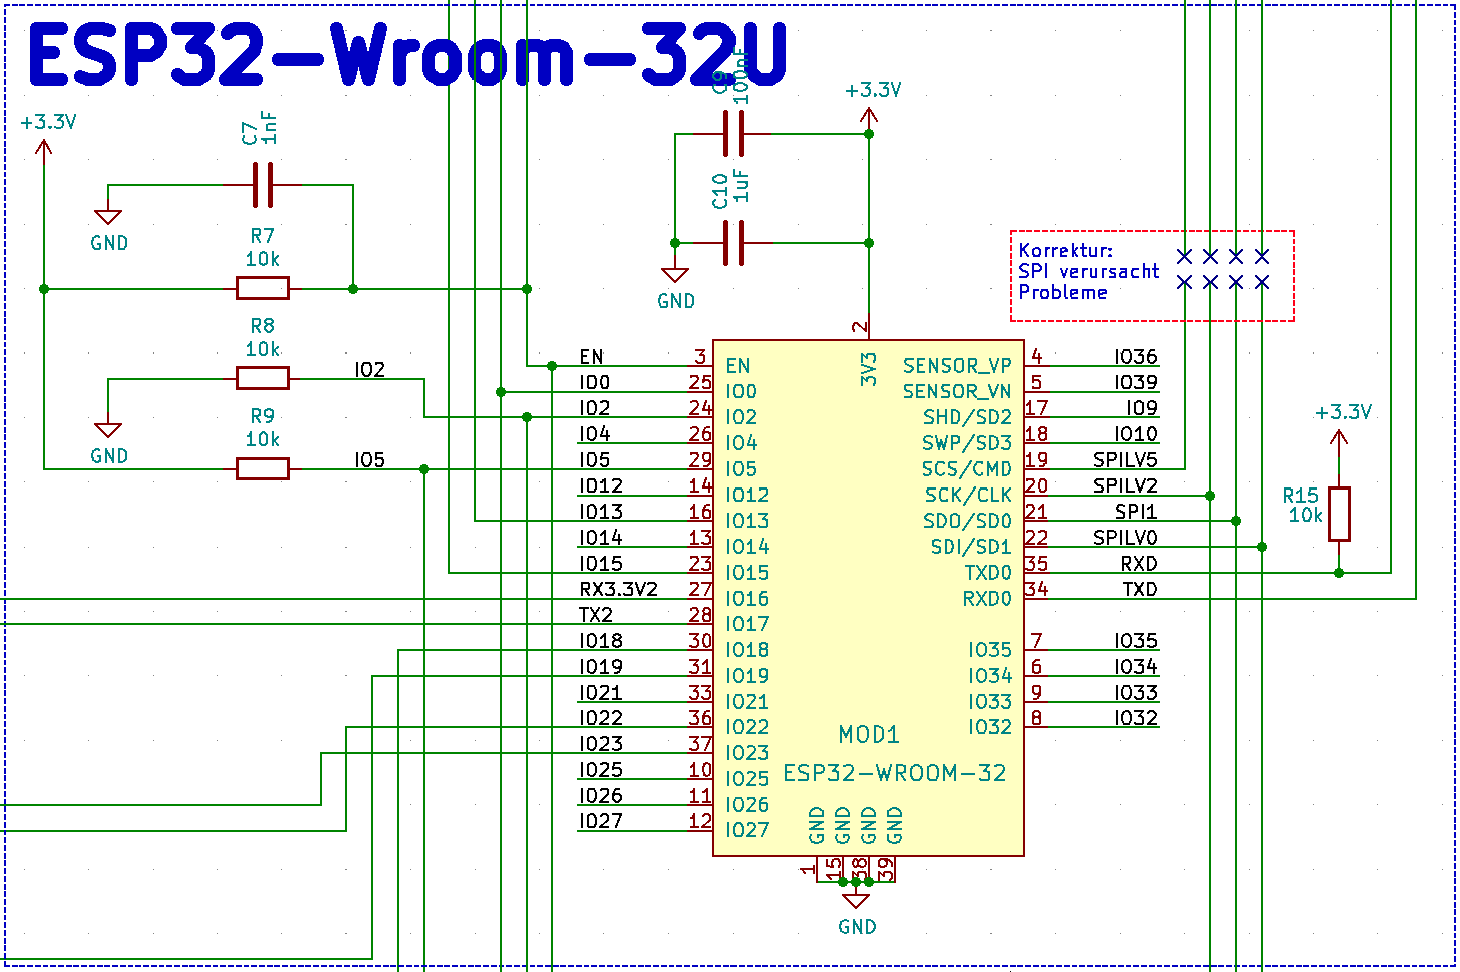
\includegraphics[width=\textwidth]{graphics/Schema_ESP32}
	\caption{Schema ESP32-Wroom-32U.}
	\label{fig:Schema_ESP32}
\end{figure}

\paragraph{Funktionsbeschrieb der Schaltung (WiFi-Modul)}\mbox{}

Das ESP32 ist mit MOD1 beschriftet, es übernimmt die in Kapitel \ref{subsec:Wirelessmodul} beschriebenen Funktionen. Die Kondensatoren C9 und C10 dienen zu Stütz- und Filterzwecken am Spannungseingang.  Über den EN-Pin wird das Modul ein- und ausgeschaltet (acitve high). Der Widerstand R7 ist ein Pull-Up für Chip-Enable. Die Widerstände R8, R9, R10 und R11 sind an die Strapping-Pins angeschlossen. Über diese werden beim Aufstarten des ESP32 der Boot-Modus, die Versorgungsspannung von VDD\_SDIO\footnote{Secure Digital Input Output}-Slave (Erweiterung der SD-Spezifikationen) und andere Initialisierungseinstellungen konfiguriert. Details zu den Konfigurationen sind in Tabelle \ref{tab:Strapping_pins} aufgelistet\footnote{https://www.espressif.com/sites/default/files/documentation/esp32\_datasheet\_en.pdf S.13}. Der Widerstand R15 zieht U0TXD auf HIGH. Aus Tabelle \ref{tab:Einfluss_Pins_auf_Boot_Modus} ist ersichtlich, dass dieser für den normalen Boot-Modus auf HIGH sein muss. Für den Download-Boot-Modus hat dieser kein Einfluss. Mit dem Kondensator C7 wird sichergestellt, dass nach einem Reset der Bootmodus gestartet werden kann. Wird der Reset-Pin au LOW gezogen, so entlädt sich der Kondensator. Sobald der Reset-Pin auf HIGH gezogen wird, dauert es länger, bis ein logic High-Zustand am CMOS-Eingang erkannt wird. Wird der Pin IO0 auf LOW gezogen, bevor der Enable-Pin nach einem Reset einen HIGH-Zustand erreicht, so wird das ESP32 in den Download-Boot-Modus gesetzt. Um automatisch in diesen Boot-Modus zu kommen benötigt es eine Logik, welche im Folgenden erklärt wird.

\paragraph{Schema (Automatische Boot-Logik)}\mbox{}

In Abbildung \ref{fig:Schema_ESP32_Flashbuttons} wird die Schaltung gezeigt, welche verwendet wird, das ESP32-Modul in den gewünschten Boot-Zustand zu bringen. Für die Beschaltung der automatischen Boot-Logik benötigt es eine Schaltung mit DTR und RTS als Inputs vom USB-UART-Converter her und EN und IO0 als Outputs auf das ESP32. Die Buttons können bei Bedarf verwendet werden, sind für den automatischen Boot-Modus jedoch nicht zwingend nötig. Sie könnten dazu verwendet werden, manuell in den Bootmodus zu gelangen.\\
Die Widerstände R20 und R21 sind Vorwiderstände an der Basis der Transistoren Q1 und Q2. R22 und R23 sind Pull-Up-Widerstände für die EN- und IO0-Leitung. Die Kondensatoren C13 und C12 dienen zum entprellen. Die Widerstände R25 und R24 begrenzen den Strom bei Drücken der Buttons S1 und S2.

\begin{figure}[h!]
	\centering
	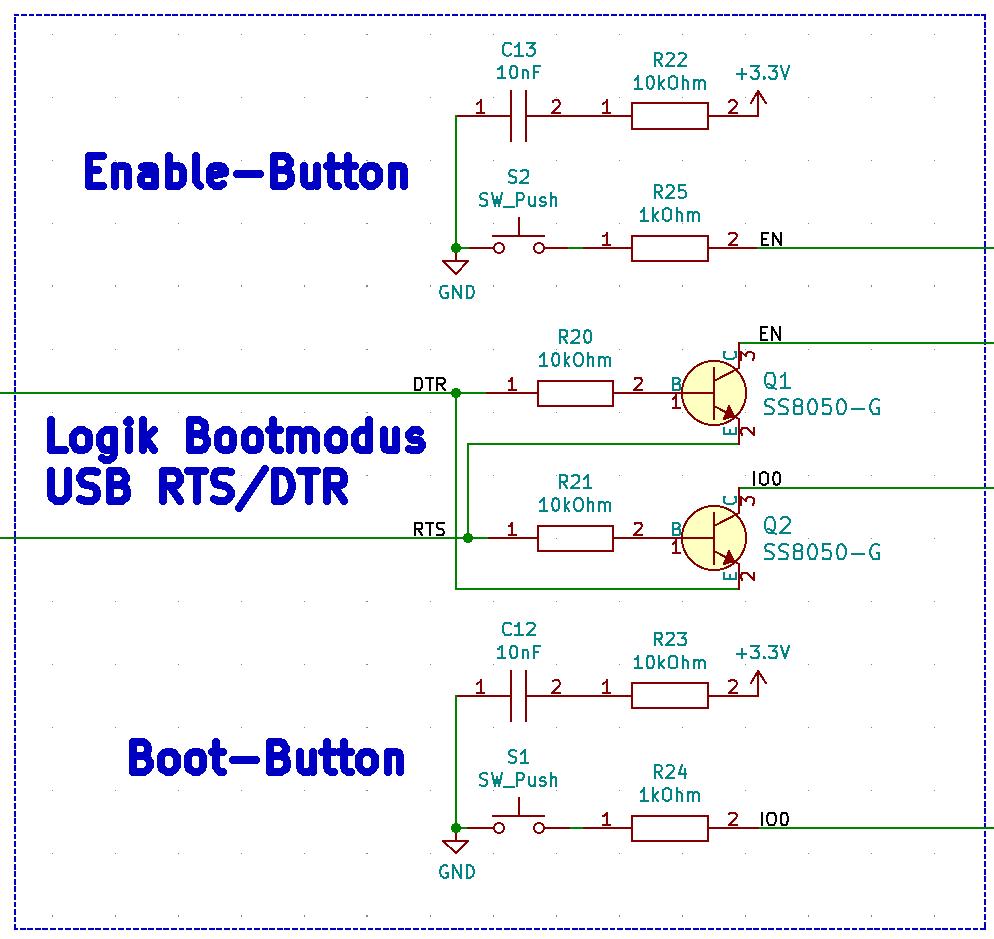
\includegraphics[width=0.7\textwidth]{graphics/Schema_ESP32_Flashbuttons}
	\caption{Schema ESP32-Wroom-32U.}
	\label{fig:Schema_ESP32_Flashbuttons}
\end{figure}

\newpage

\paragraph{Funtionsbeschrieb der Schaltung (Automatische Bootlogik)}\mbox{}

